%%%
%% Specification :: Scope
%%%
\section{Scope}

%%%
%% Specification :: Scope :: Organisation Structure
%%%
\subsection{Organisation Structure}

The project team is based largely upon democratic discussions and decisions,
however to ensure that team deadlocks do not occur a project leader has been
chosen. Figure ~\ref{fig:org_hierachy} reflects the hierarchy of the team.

\begin{figure}[H]
  \centering
  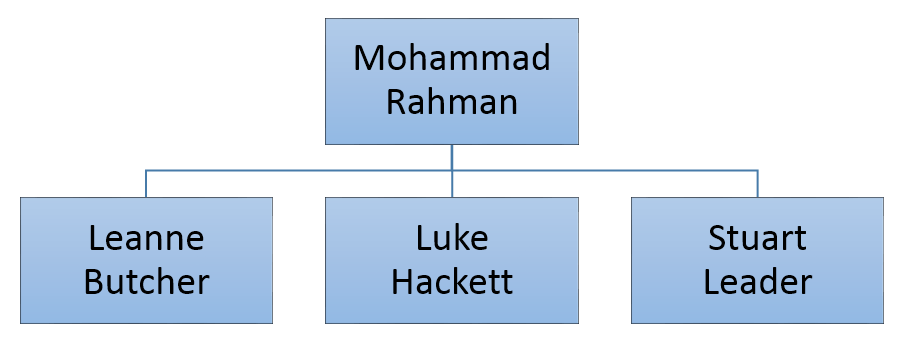
\includegraphics[width=0.9\textwidth]{organisation_structure.png}
  \caption{Hierarchical Structure of the team}
  \label{fig:org_hierachy}
\end{figure}


%%%
%% Specification :: Scope :: Organisation Structure :: Methodology
%%%
\subsection{Methodology}

It has been decided that the team will follow an Agile software development
model. This will allow the team to split the larger task down into smaller, more
manageable `chunks', that allows for a good quality analysis, evaluation,
development and planning (on to the next `chunk'). An iterative approach is best
suited for this project due to the nature of changes and updates the product
will require in future builds.

This method of development also allows for a more feature-driven approach to the
project. Ultimately this allows for more important features and aspects of the
project to be completed first.


%%%
%% Specification :: Scope :: Meetings
%%%
\subsection{Meetings}

A weekly meeting will take place between all project members to discuss all
aspects of the project. This includes (but is not limited to) project issues,
software development issues, research findings, possible improvements and code
reviews.


%%%
%% Specification :: Scope :: Product
%%%
\subsection{Product}

Within the cryptic crossword area, there is a need for a cryptic crossword clue
solver in the form of a software application.  This has been justified
previously within the document through research and investigating existing
applications within the field. The main purposes of the software deliverable are
to allow the input of a cryptic crossword clue by a user and output a potential 
results or number of results.

Once the project has been completed by the team, the following deliverables will
have been accomplished:

\begin{itemize}
  \item A software application which accepts input from the user and outputs 
        appropriate solutions. 
  \item Two written reports that:
    \begin{itemize}
      \item document the entire software development process from a group 
            perspective
      \item analyse and evaluate the project as a whole
    \end{itemize}
\end{itemize}

Furthermore the subsequent internal components will be implemented to aid with 
the goals of the project:

\begin{itemize}
  \item A storage area to collect and store the cryptic crossword clues and 
        their details used for test data as well as, clues successfully solved 
        by the application which a user has input.
  \item A service which will allows connections from web browsers and 
        potentially mobile phones to ensure the running of the software 
        application.
\end{itemize}

There are specific criteria which have been identified as important features
which must be completed to deem the project as adequately finished:

\begin{itemize}
  \item A document outlining the full software development life cycle of the 
        project
  \item A software application which can be accessed via either:
    \begin{itemize}
      \item A web browser \textbf{and/or}
      \item A portable device (e.g. smartphone or tablet)
    \end{itemize}
  \item A service which can be connected to by either a mobile phone or a web 
        browser which will sufficiently solve a cryptic crossword clue and 
        output a result or number of results 
  \item A storage area accessible by the service which stores the cryptic 
        crossword clues and their associated details
\end{itemize}

Furthermore, there are specific criteria which have been deemed as out of the 
scope of the project:

\begin{itemize}
  \item The user will not be able to access the storage area to browse through 
        data
  \item The software application will not be implemented to have the ability to
        generate cryptic crosswords from the data stored
\end{itemize}

The restrictions listed below are the justifications for the project scope:

\begin{itemize}
  \item The time scale of the project
  \item External priorities from the academic year such as other module 
        assignments and examinations
  \item Limited resources for testing the software application on restrict the
        platforms which the software application will be fully compatible with
\end{itemize}
